In this chapter the website and it's functions are described. Furthermore, there will be some explanation about the logic that drives the website.

\section{Reason of existence}
The website is the place where the online speakers and objects are manipulated.
The idea of the website is to enable the user to simply drag and drop speakers/objects with platform independency in mind.
The website had to be simple, easy to use and not dependent of some kind of webserver.
So the website has to be portable\footnote{Platform independent, eg usable on Linux, Windows, etc...}.
For this reason the website's main logic is made in JavaScript and The layout with simple HTML and a small hint of CSS which was used to bring it all up to flavor.
Most web browser's can open the website, the \textit{index.html} file, and see the site and online speakers.

\section{Challenges}
Some challenges that where faced when making this website. Some where small and some where big. {\tiny\textit Insert Yo Momma Joke}

\subsection{MQTT with web sockets}
This website needs to connect to an MQTT broker. Because of the rule of platform independency and portability, some kind of connectivity with JavaScript is needed.
Enter the world of web sockets! For this project, the \href{https://github.com/eclipse/paho.mqtt.javascript}{Paho JavaScript Client} is used.
The Paho JavaScript Client is an MQTT browser-based client library written in JavaScript that uses Web Sockets to connect to an MQTT Broker.

\subsection{Website flow}
In figure \ref{fig:website_flow} is the startup and flow sequence of the website displayed.
When the site comes online, the unknown dataset\footnotemark first has to be rebuild.
\footnotetext{The dataset is all the online clients with all the objects and their information. See \hyperref[clients]{clients} of the \hyperref[chap:Topics]{topics chapter}}
After this initialisation, the website is in it's main \textit{"flow"}. From here the site has three possibility's:
\begin{itemize}
    \item User interacts with the drawing (speakers/objects)
    \item Site got new speaker data (from a single speakers)
    \item Site got complete new dataset
\end{itemize}
In the \hyperref[chap:Topics]{topics chapter}, are the topics defined that are used to send and receive the data to and from all the devices.

\begin{figure}[H]
    \centering
    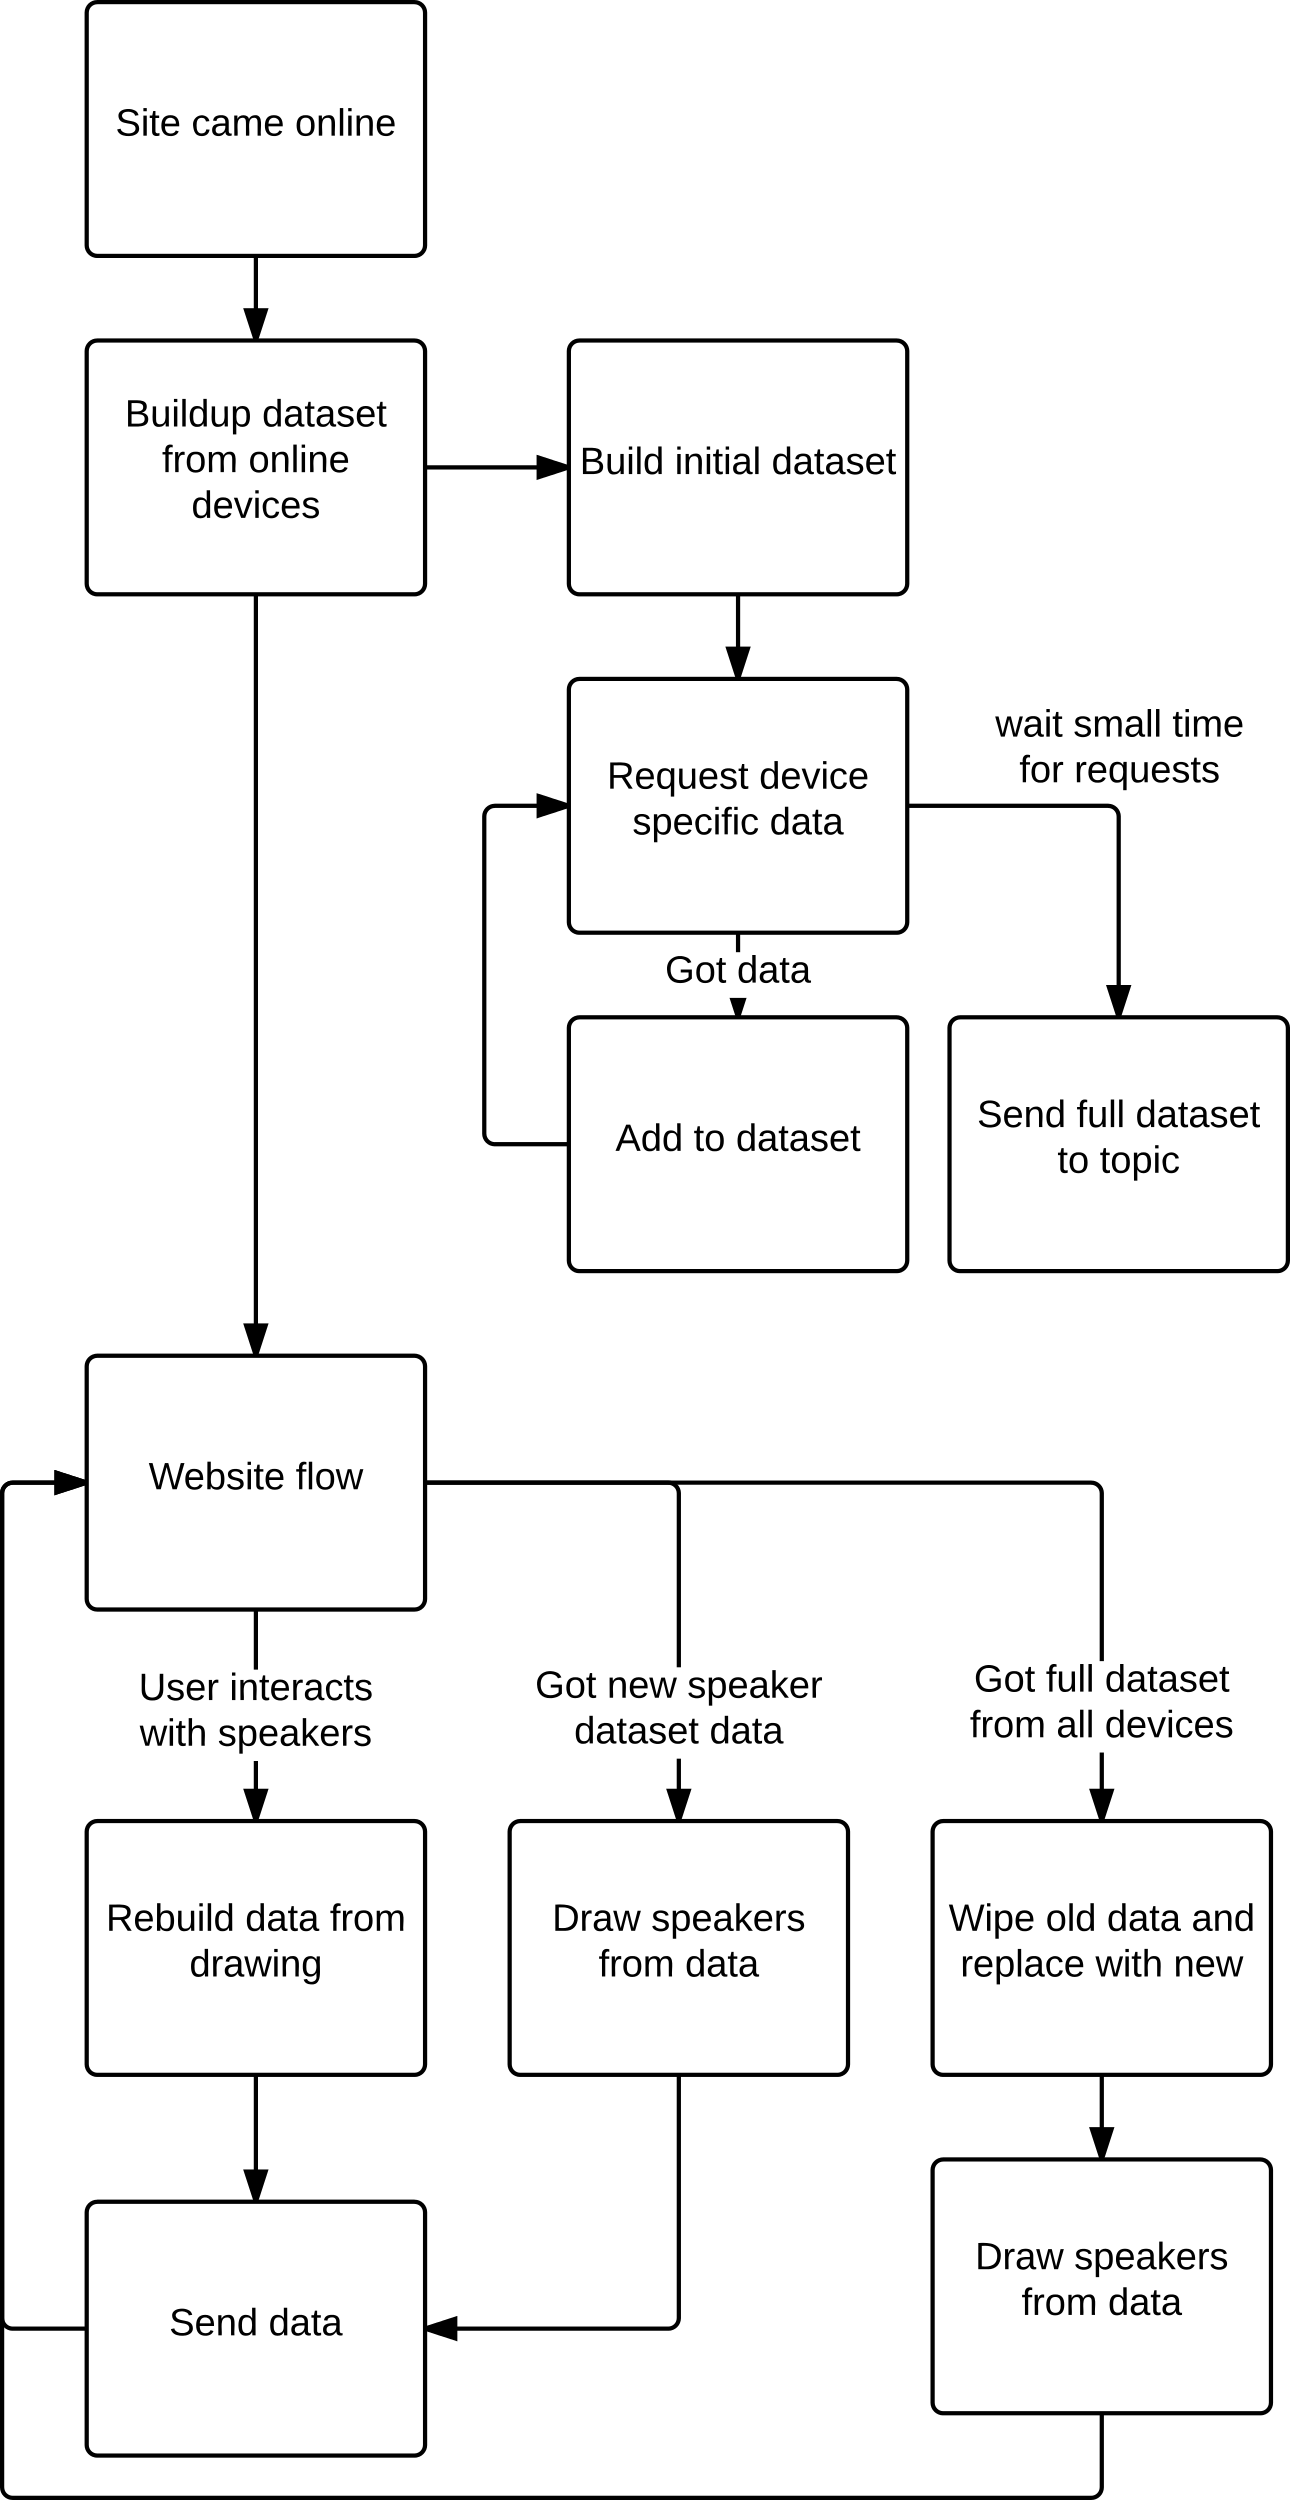
\includegraphics[height=.5\paperheight]{website_flow}
    \caption{The flow of the website}
    \label{fig:website_flow}
\end{figure}

\subsection{Draw and synchronize objects}
To draw and synchronize the drawn speakers/objects, there are three features needed.
One that will draw all the available speakers and objects from the dataset,
one that will generative said dataset from the drawn objects and speakers
and a way of synchronizing this data between website and speaker.

\subsubsection{Draw speakers from data}
To draw the speakers and objects, the dataset is needed. This dataset holds all the data that is needed for the drawing.
This data holds all the relations between the speakers and the objects.
As seen in figure \ref{fig:website_draw_from_data}, it will simply be a looping scheme.
In this diagram, a somewhat crude software architecture is demonstrated.
The drawing is started from an object, and with all the data that is known, the rest is draw.

Because this is a simple 2D field, all the drawn speakers, will contain all the drawn objects.
I.e. if there are two objects(obj1, obj2) and two speakers(sp1,sp2), sp1 will contain the distance and angle from sp1 to obj1 and ob2.
Sp2 in this example will also have this data, not the same values of course, but it will have the distance and angle from sp1 to obj1 and obj2.
With this knowledge, it is only needed to draw an object or speaker once and after that it is not needed to check if the remaining data of that object correlates with the data of another speaker.
In this case, it is assumed that the data represents a single 2D drawing area.

\begin{figure}[H]
    \centering
    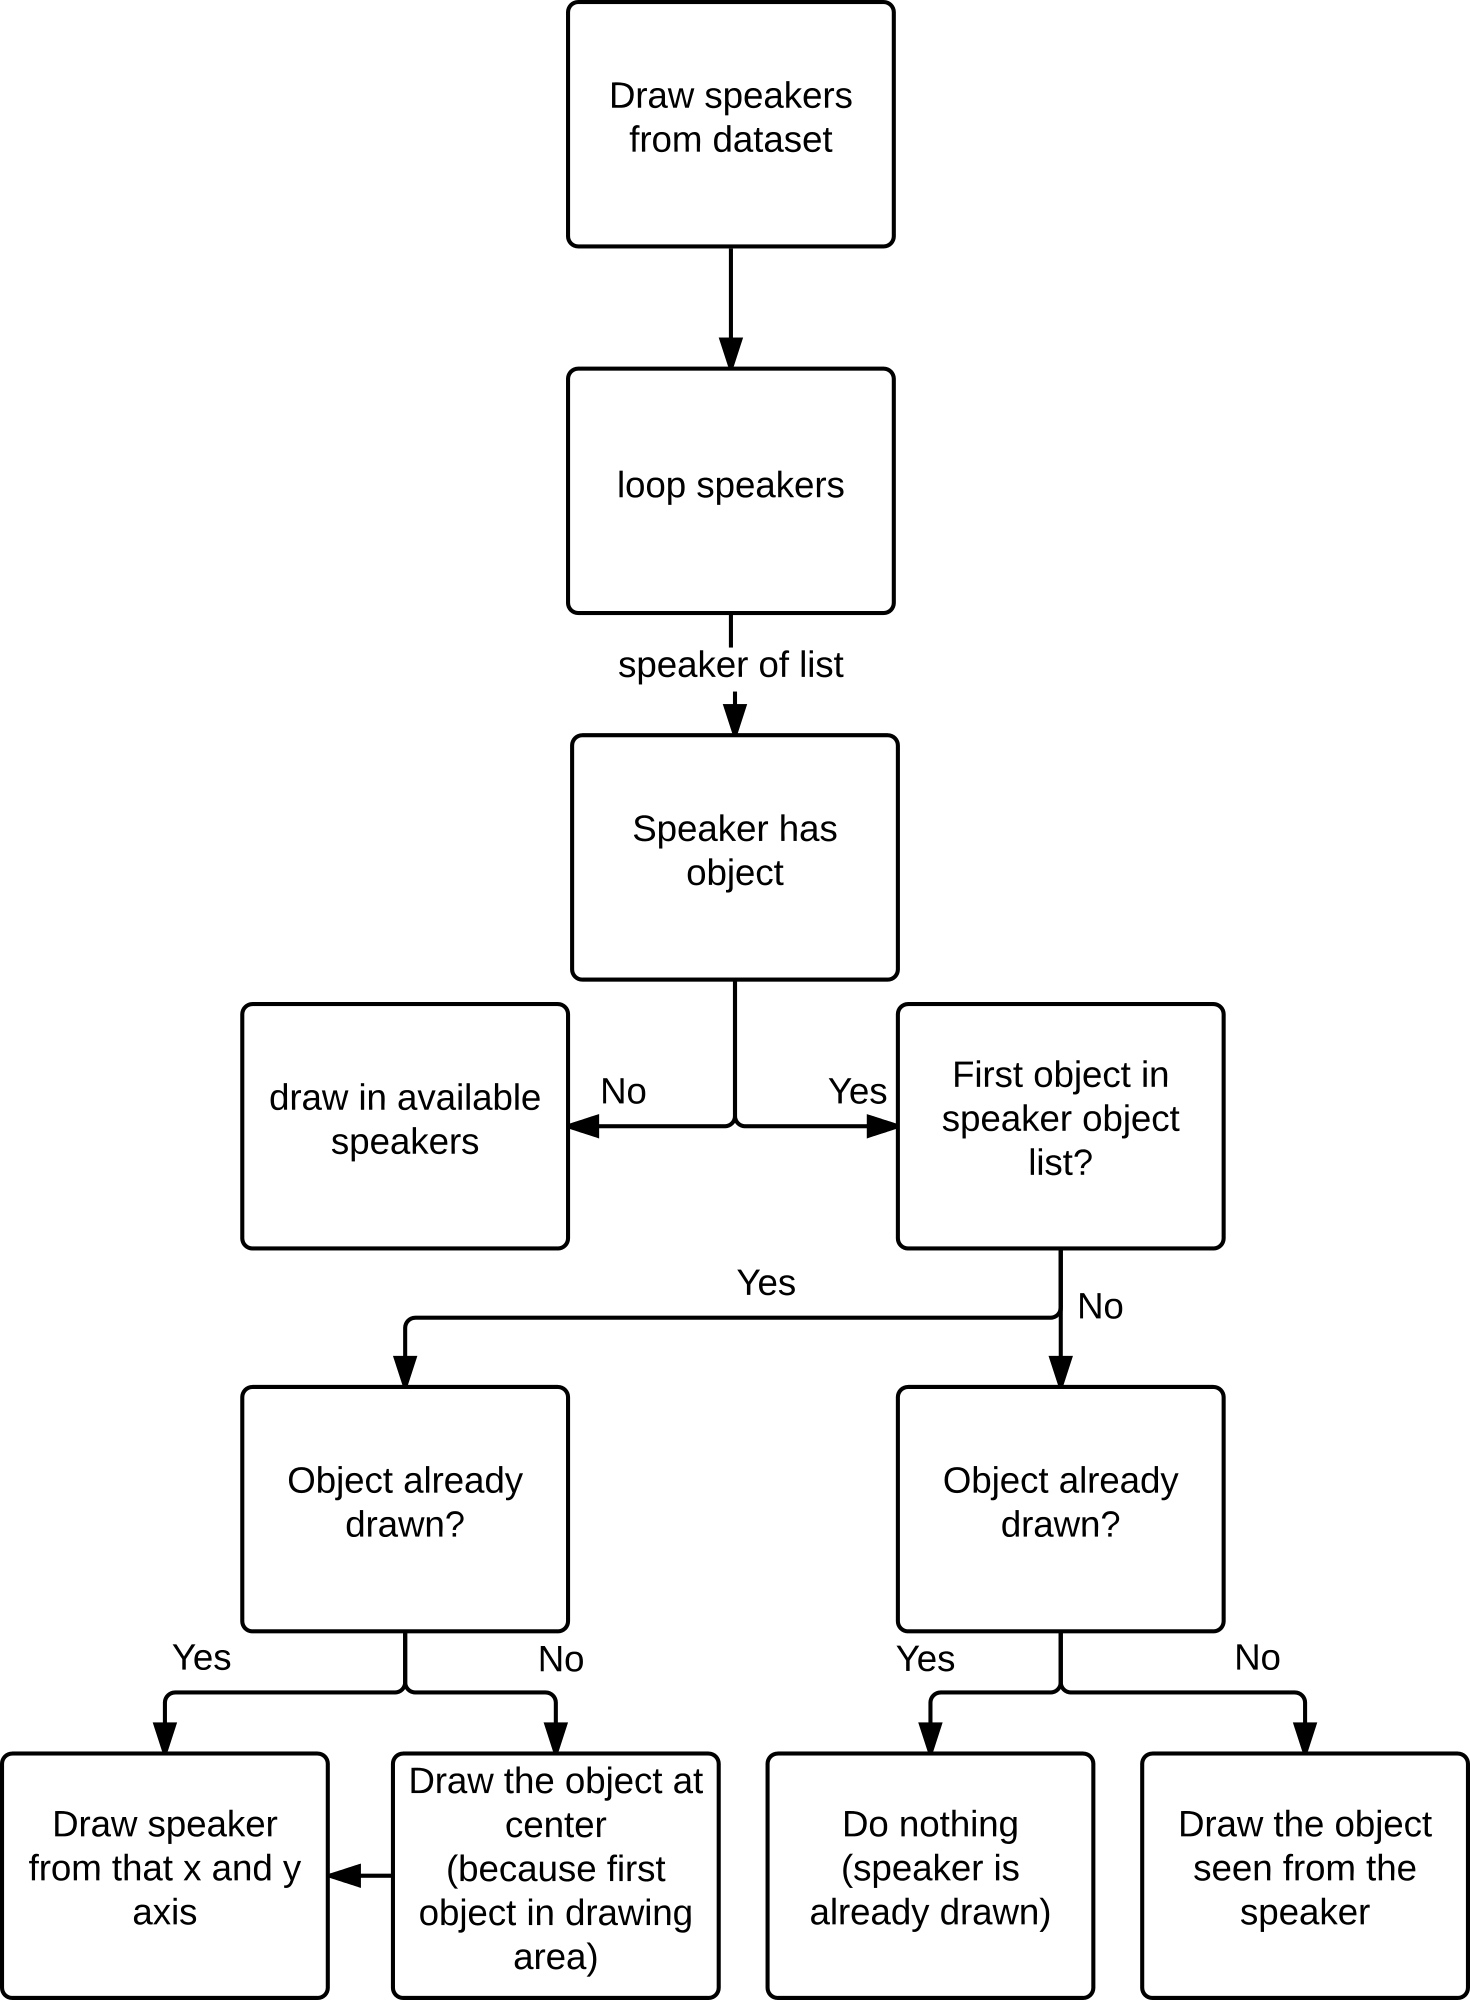
\includegraphics[height=.5\paperheight]{website_draw_from_data}
    \caption{Draw speakers and objects from the dataset}
    \label{fig:website_draw_from_data}
\end{figure}

\subsubsection{Generate dataset from drawing}
This feature has a simple task. Loop all speakers and calculate all the distances and angles from speaker to the objects.
Figure \ref{fig:website_make_data_from_drawing} describes this quite well.

\begin{figure}[H]
    \centering
    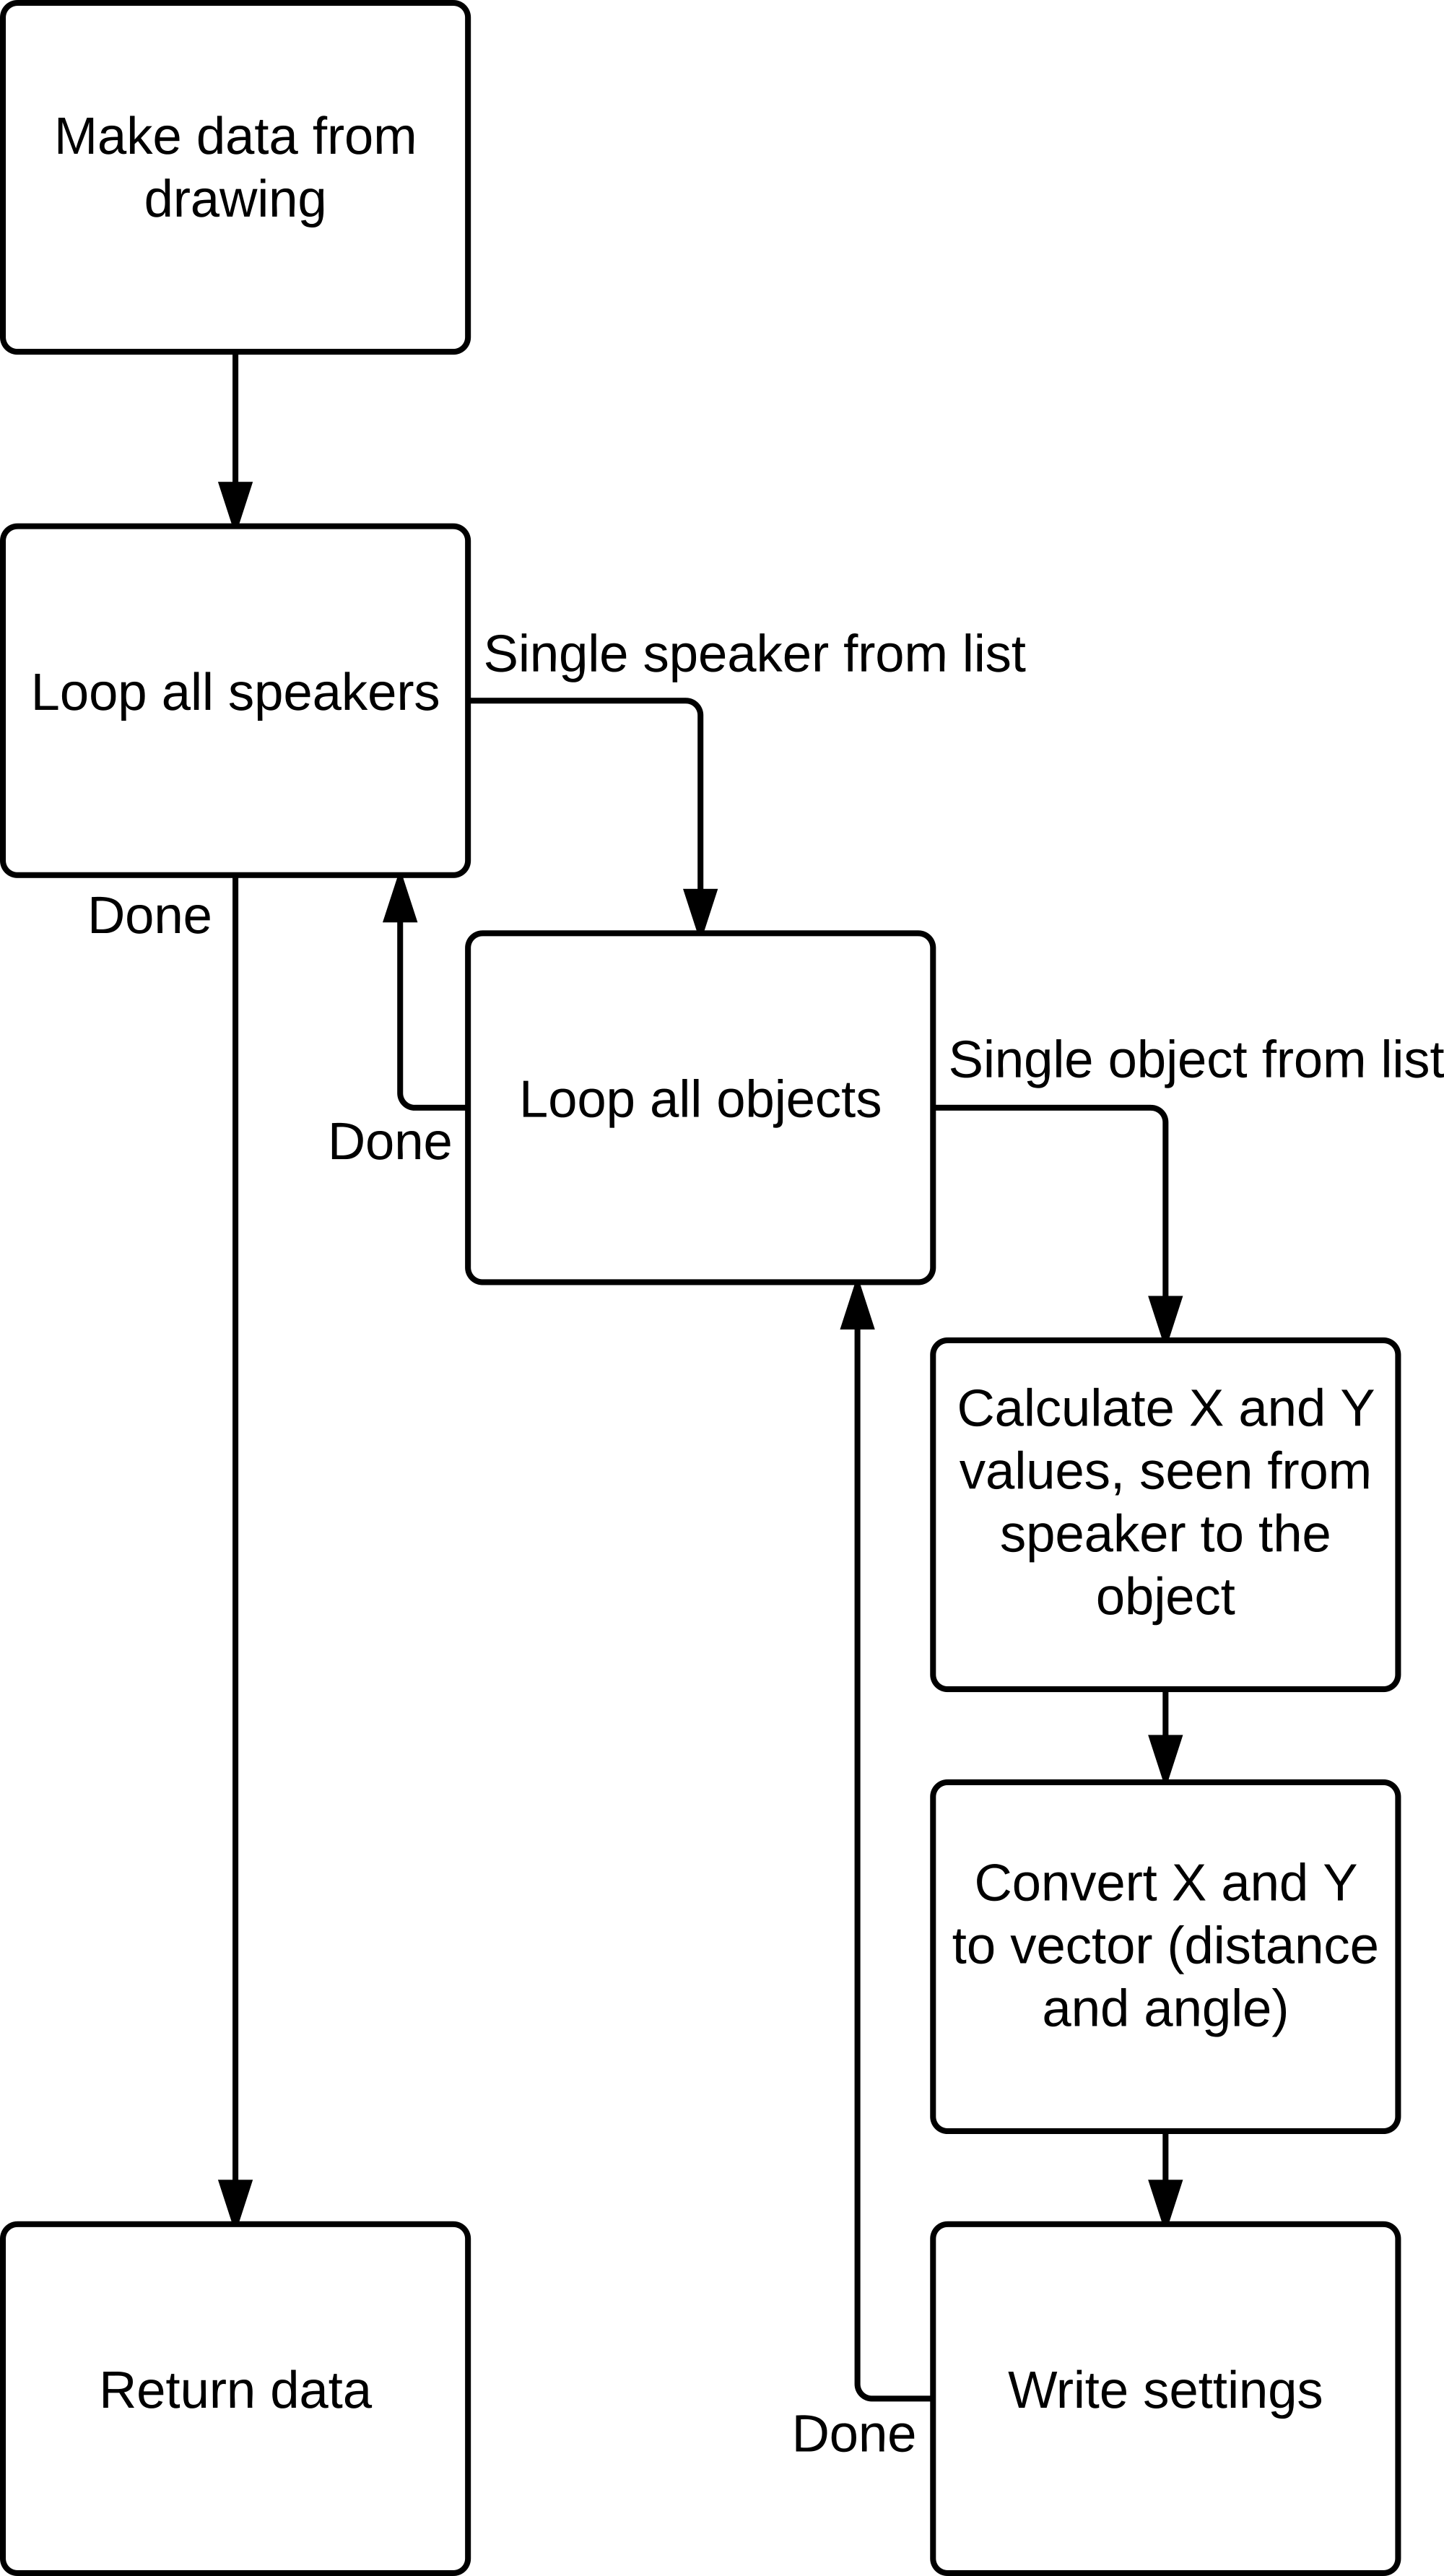
\includegraphics[height=.5\paperheight]{website_make_data_from_drawing}
    \caption{Generate the dataset from the drawing}
    \label{fig:website_make_data_from_drawing}
\end{figure}

\subsubsection{Synchronization}
The last part is the synchronization. This is used for a synchronization between two or more websites and clients.
The dataset is generated.
The moment this is send to the clients, the other website(not the one sending), will also fetch this data and use this to draw the objects.
One extra topic is used in this system specific for the website.
The moment, a website send this data, it also send the x and y offset of the first drawn object.
This way, there is a reasonable failsafe system with the least amount of overhead\footnotemark.
\footnotetext{An other solution would be to send the complete dataset for websites, but instead of distances and angles, x and y values/offsets.
This is not the best solutions, because what happens if the offset message isn't send?
The drawing will be drawn from the middle instead of the other website's x and y offset.
This would ensure that the syncing issue would not be happening.
But this means that for x messages to the clients, x messages to the websites need to be send}

\subsection{Loading configuration file\\
    \small\nimbus\textit{The not so beautiful approach}}
In this system, a single configuration file is used between website and client.
This file contains all sorts of data.
In JavaScript there is however a problem with this setup. In C or C++ this would be easy, just read it from the local file system.
In general, this is not allowed in JavaScript by design. It's a violation of the sandbox.
There are API's to load a file via a button etc, but this is not user friendly.
Think about it, every time the site is loaded, a window pop's up with the message:
\say{Hello dear user, would you please be kind and load a config file. If you don't, I will not work.}.

The solution was to load this config file on load time. Just like any other JavaScript file is loaded via the script src tags.
The config file was saved with a \say{.js} extension, started with: \say{var CONFIG =} and ended with \say{;}.
The client can filter this out and the website can load in the config file.

It is a solution, maybe not the best, but it works.

\section{Website layout}
In these following paragraphs, the layout and main usage of the site is explained.

\subsection{Idle}
In figure \ref{fig:website_idle} is the state of the website shown when it is in idle mode.
On the right hand side are the available speakers and objects. From here, the user can drag these in the draw area.

\begin{figure}[H]
    \centering
    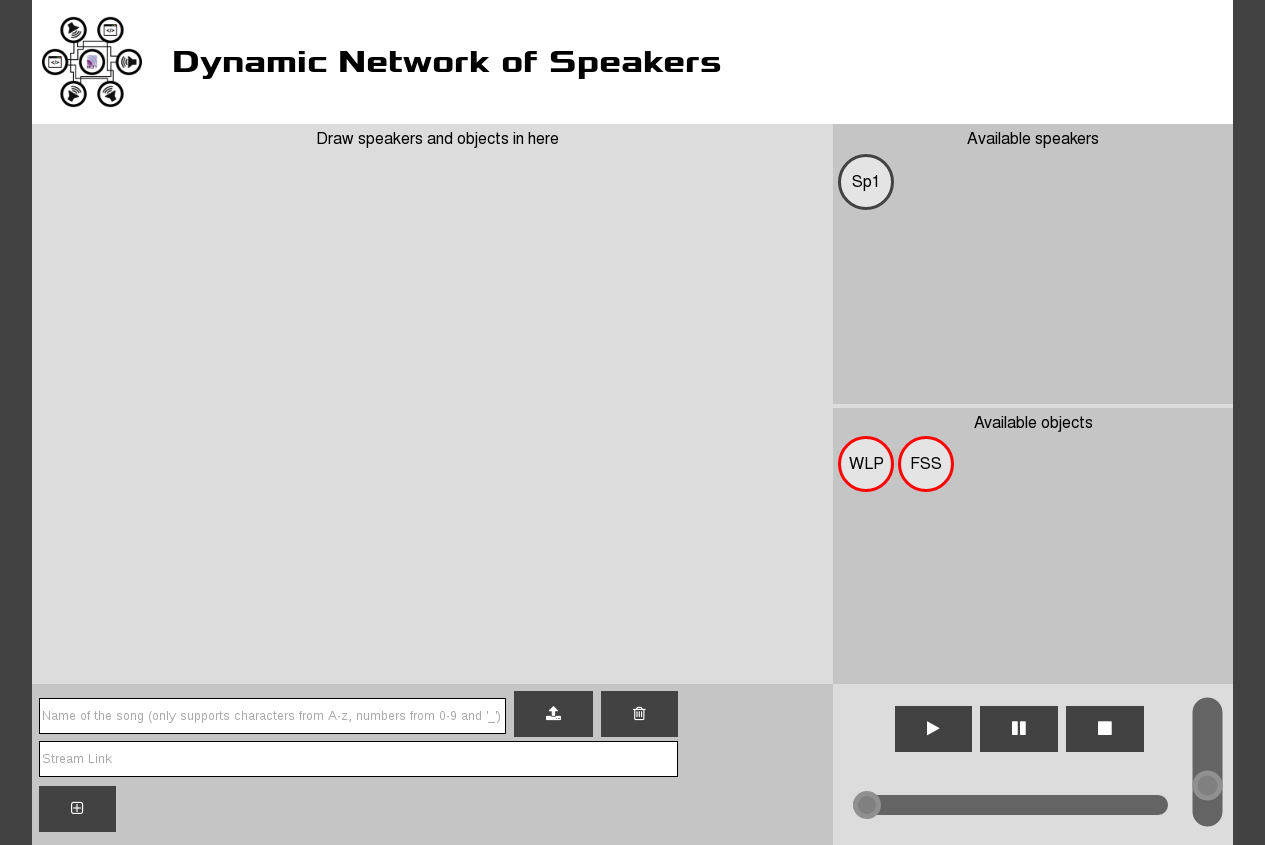
\includegraphics[width=.8\textwidth]{website_idle}
    \caption{Website when idle}
    \label{fig:website_idle}
\end{figure}

\subsection{Manipulating speakers and objects}

Demo of usage, one and two objects.
\begin{figure}[H]
    \centering
        \begin{minipage}[b]{0.5\textwidth}
            \centering
            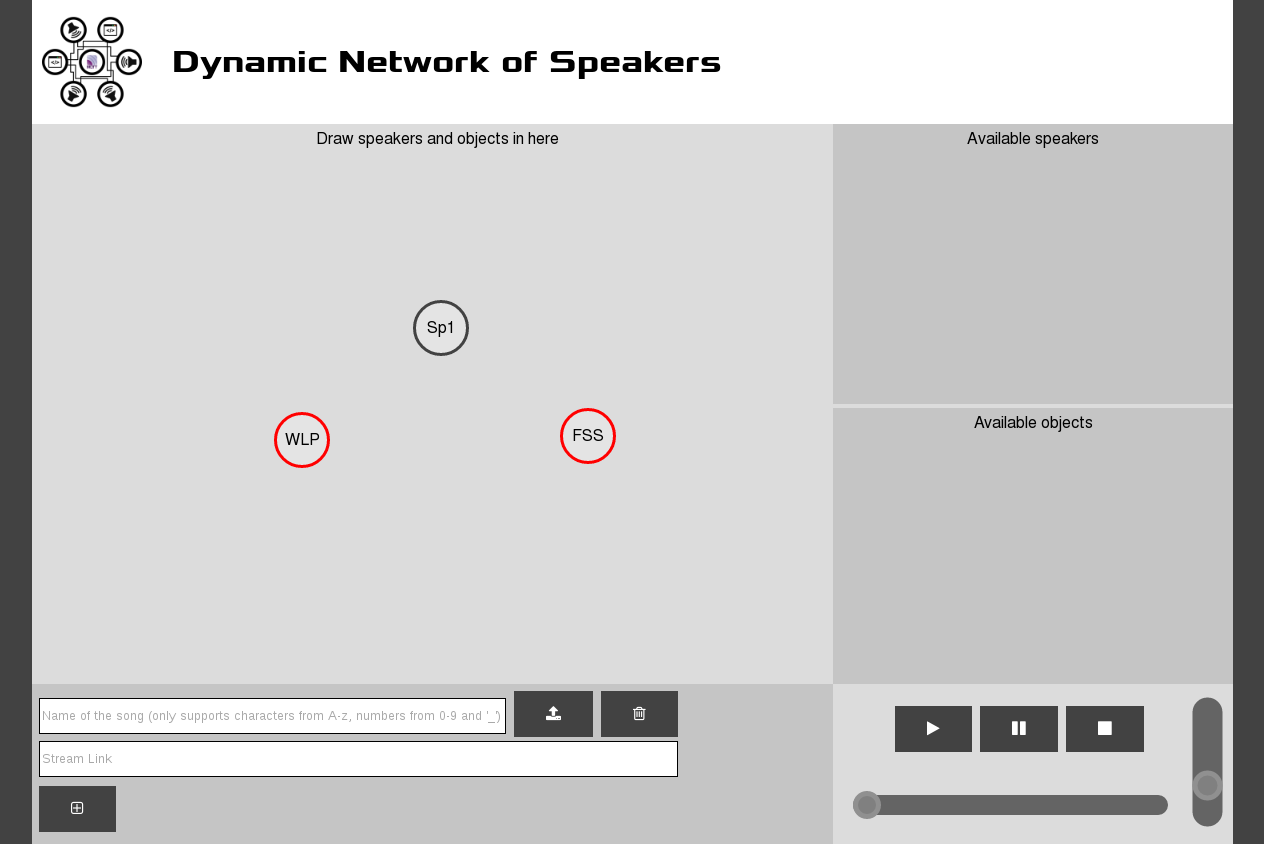
\includegraphics[width=.9\textwidth]{website_1sp_2obj}
            \caption{One speaker and two objects}
            \label{fig:website_1sp_2obj}
        \end{minipage}%
        %
        \begin{minipage}[b]{0.5\textwidth}
            \centering
            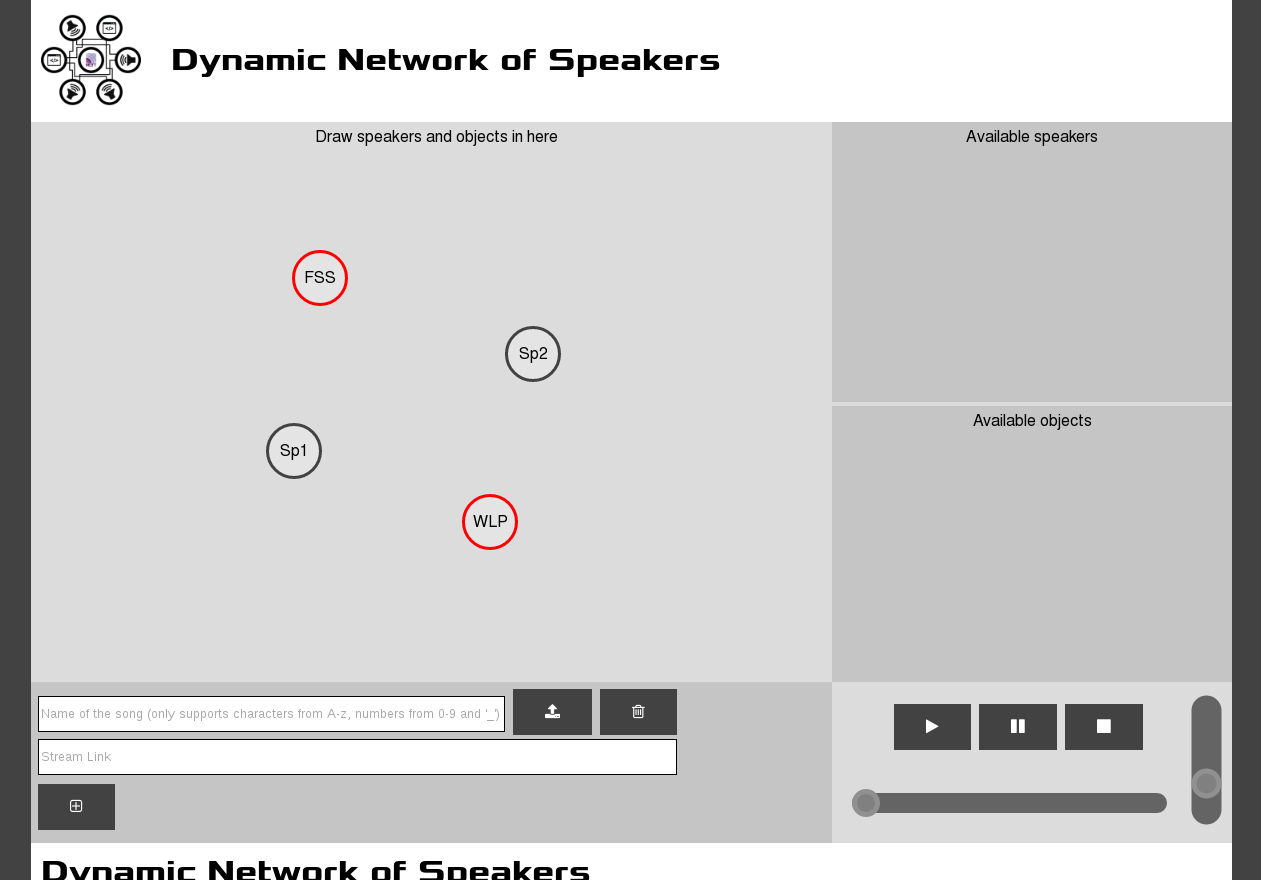
\includegraphics[width=.9\textwidth]{website_2sp_2obj}
            \caption{Two speakers and two objects}
            \label{fig:website_2sp_2obj}
    \end{minipage}
\end{figure}

\subsection{Edit objects}

Edit objects
\begin{figure}[H]
    \centering
    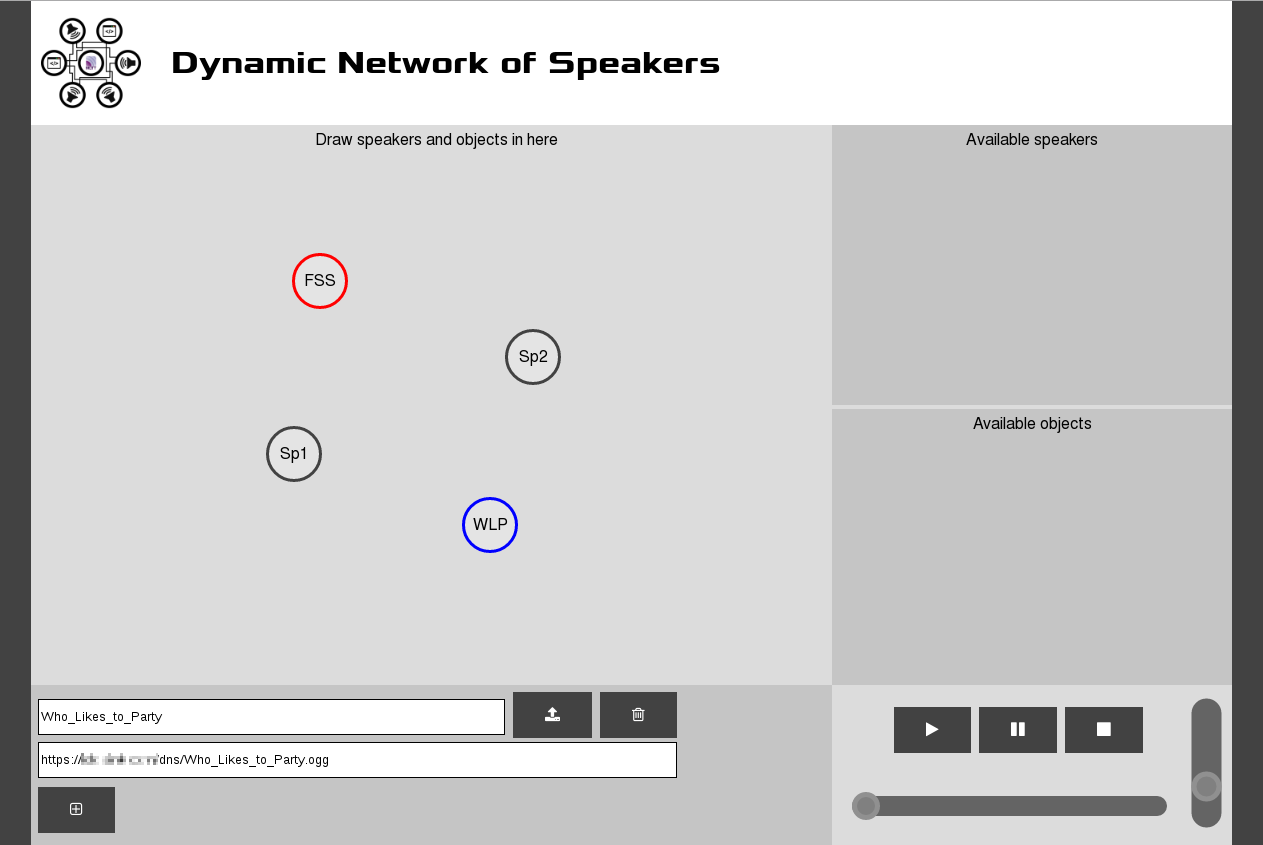
\includegraphics[width=.8\textwidth]{website_edit_object}
    \caption{Edit an object}
    \label{fig:website_edit_object}
\end{figure}

\subsection{Extra options}
Extra options

\begin{figure}[H]
    \centering
    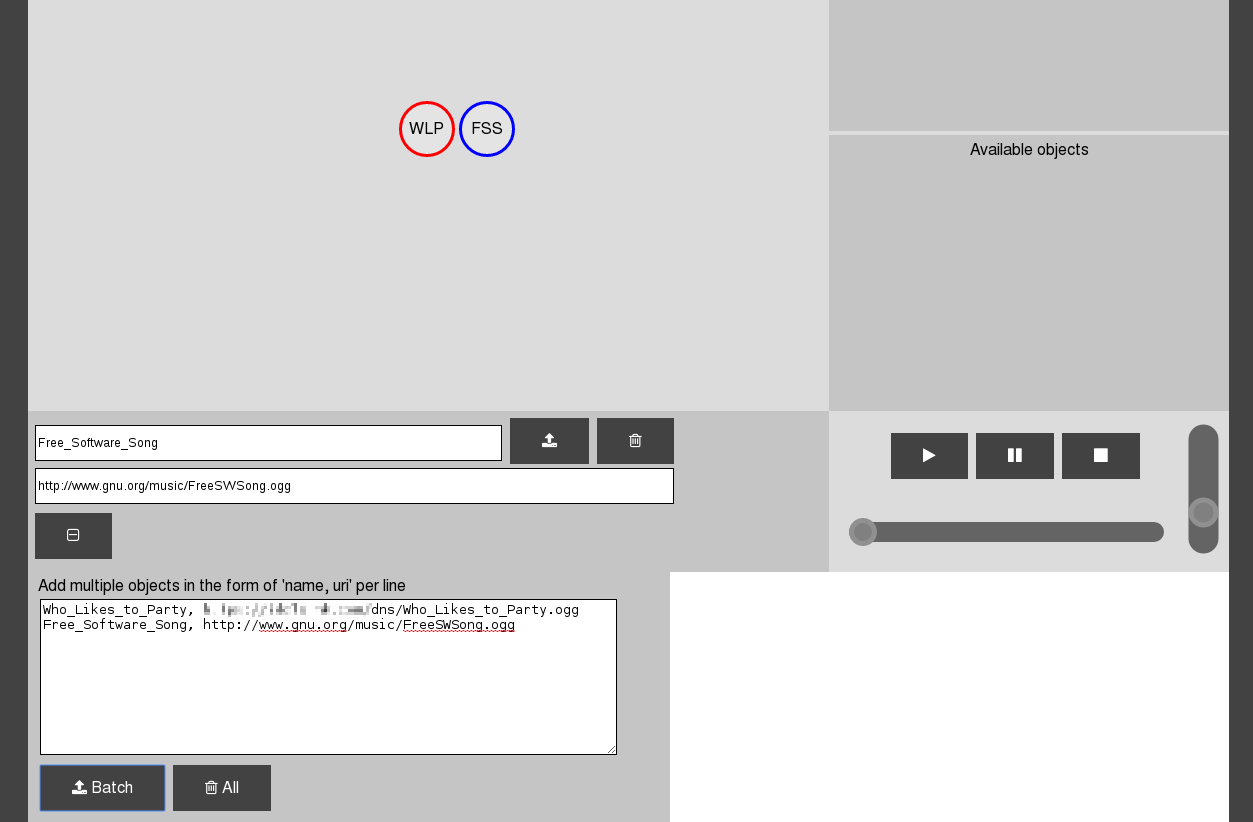
\includegraphics[width=.8\textwidth]{website_extra_options}
    \caption{Extra options}
    \label{fig:website_extra_options}
\end{figure}
